\documentclass[letterpaper,10pt,titlepage]{article}

\usepackage{graphicx}                                        
\usepackage{amssymb}                                         
\usepackage{amsmath}                                         
\usepackage{amsthm} 
\usepackage{verbatim}                                         

\usepackage{alltt}                                           
\usepackage{float}
\usepackage{color}
\usepackage{url}
\usepackage{fancybox}
\usepackage{verbatim}

\usepackage{balance}
\usepackage[TABBOTCAP, tight]{subfigure}
\usepackage{enumitem}
\usepackage{pstricks, pst-node}
\usepackage{texments}

\usepackage{geometry}
\geometry{textheight=9in, textwidth=6.5in}

\newcommand{\cred}[1]{{\color{red}#1}}
\newcommand{\cblue}[1]{{\color{blue}#1}}
\newcommand{\tab}{\hspace*{2em}}

\usepackage{hyperref}
\usepackage{geometry}

\def\name{Eric Timmerman, Stephanie Ison, Geoffrey Corey}

%% The following metadata will show up in the PDF properties
\hypersetup{
  colorlinks = true,
  urlcolor = black,
  pdfauthor = {\name},
  pdfkeywords = {cs325 ``algorithmic analysis''},
  pdftitle = {CS 325: Project 1},
  pdfsubject = {CS 325: Project 1},
  pdfpagemode = UseNone
}

\begin{document}
\hfill \name

\hfill \today

\hfill CS 325 Proj 1

\section{Run-time Analysis}
\subsubsection{Enumeration 1}
Let $0$ to end be $n$\\
Let the index be $k$\\
First loop = $n$ amount of work\\
the second for loop = $n - k$ amount of work\\
Which = $n(n-k)$\\
$n(n-k) = n^{2}-nk$\\
$\lim_{n \rightarrow \infty} n(n-k) = n^{2}-nk \leq n^{2}$\\
Therefore, Enumeration 1 is $O(n^{2})$

\subsubsection{Enumeration 2}
Let $0$ to end be $n$\\
Let $index$ be $j$\\
The first for loop = $m$ amount of work\\
The second for loop = $\frac{(m-j)}{2}$ amount of work\\
the third for loop = $\frac{(m-j)}{2}$ amount of work\\
This is close to $m(m-j)$\\
$m(m-j) = m^{2}-mj$\\
$\lim_{n \rightarrow \infty} m(m-j) = m^{2}-mk \leq m^{2}$\\
Therefore, Enumeration 2 is $O(m^{2})$

\subsection{Pseudo-code}
\subsubsection{Enumeration 1}
enumeration1(list)\\
\tab{$minimum = \infty$}\\
\tab{$total = 0$}\\
\tab{for $i$ in $list$}\\
\tab{\tab{$total = 0$}}\\
\tab{\tab{for $j$ from $i$ to end of $list$}}\\
\tab{\tab{\tab{$total += list[j]$}}}\\
\tab{\tab{\tab{if \(\lvert $total$\rvert\) $< minimum$}}}\\
\tab{\tab{\tab{\tab{$minimum =$ \(\lvert$total$\rvert\)}}}}\\
\tab{\tab{\tab{\tab{$left = i$}}}}\\
\tab{\tab{\tab{\tab{$right = j$}}}}\\
\tab{return $i,j$}\\\\

\subsubsection{Enumeration 2}
enumeration2(list)\\
\tab{$minimum = \infty$}\\
\tab{$total = 0$}\\
\tab{$dir = right$}\\
\tab{for $i$ in $list$}\\
\tab{\tab{if $dir = right$}}\\
\tab{\tab{\tab{$total = 0$}}}\\
\tab{\tab{\tab{for $j$ from $i$ to end of $list$}}}\\
\tab{\tab{\tab{\tab{$total += list[j]$}}}}\\
\tab{\tab{\tab{\tab{if \(\lvert$total$\rvert\) $< min$}}}}\\
\tab{\tab{\tab{\tab{\tab{$min =$ \(\lvert$total$\rvert\)}}}}}\\
\tab{\tab{\tab{\tab{\tab{left = $i$}}}}}\\
\tab{\tab{\tab{\tab{\tab{right = $j$}}}}\\
\tab{\tab{if $dir = left$}}\\
\tab{\tab{\tab{for $j$ from end of $list$ to $i$}}}\\
\tab{\tab{\tab{\tab{$total += list[j]$}}}}\\
\tab{\tab{\tab{\tab{if \(\lvert$total$\rvert\) $< min$}}}}\\
\tab{\tab{\tab{\tab{\tab{$min =$ \(\lvert$total$\rvert\)}}}}}\\
\tab{\tab{\tab{\tab{\tab{left = $i$}}}}}\\
\tab{\tab{\tab{\tab{\tab{right = $j$}}}}\\
\tab{\tab{$dir = !dir$}}\\
\tab{return $i,j$}

\subsection{Asymptotic Analysis}
\subsubsection{Enumeration1}
\subsubsection{Enumeration2}

\section{Experimental Analysis}
\verbatiminput{plotting.txt}
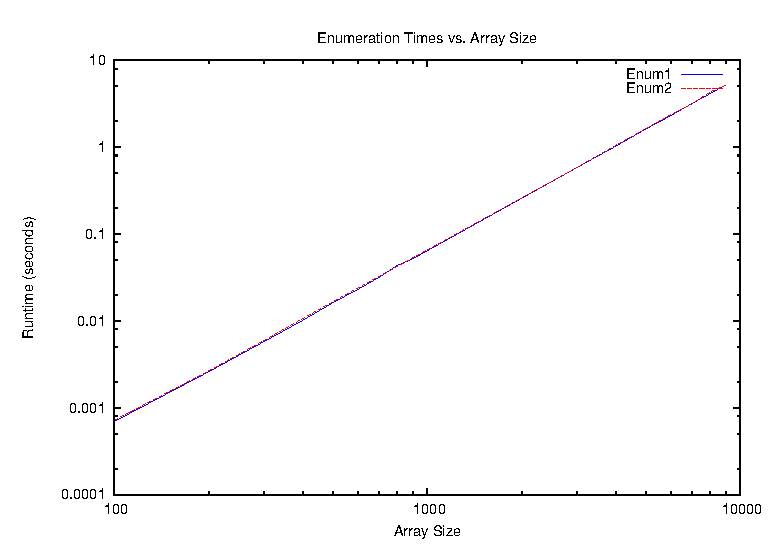
\includegraphics[width=\textwidth]{graph.eps}


\section{Extrapolation and interpretation}
\subsection{Length to Process for 1 Hour?}
Using
\begin{equation}\label{eq:Slope}
Slope = m = \frac{log(\frac{F_{1}}{F_{0}})}{log(\frac{x_{1}}{x_{0}})}
\end{equation}

Using \eqref{eq:Slope} to get the slope of enum1, I get $1.96504$. Plugging this value back into the slope equation and using $3600$ for one of the $x$ values,
\begin{equation*}
1.96504 = \frac{log(\frac{0.000696}{3600})}{log(\frac{100}{x})}
\end{equation*}
and solving for the only $x$ value shows that and array of length $260,958$ should require $1$ hour to process. And since both the enum1 and enum2 plots are very similar, the length of an array to require a processing time of 1 hour for enum2 would also be extremely close to $260,958$.

*used \url{http://en.wikipedia.org/wiki/Log-log_plot} for help understanding log slope.
\subsection{Discrepancies Discussion}
\subsubsection{Log Plots}

Using \eqref{eq:Slope} I get that the slope of enum1 is $1.96504$.

\begin{equation}\label{eq:Function}
F(x) = C * x^{m}, C = constant
\end{equation}

After finding the slope, enum1 is $C * x^{1.96504}$ from using \eqref{eq:Function}, which roughly matches with the $O(n^{2})$.

\subsubsection{Discrepancies}
Since both enumeration methods had extremely similar results, the expected asymptotic analysis for the intent of the 2nd enumeration method is different than what we found.

Also, there is a slight discrepancy between the asymptotic analysis of the first enumeration method and the results from the experiment ($1.96504 \neq 2$) because of slight differences in the programming language as well as difference in how and what the computer was running at the time of the tests. However, this was minimized by taking the average of 10 runs for each array size to account for this fluctuation.


\end{document}
